\documentclass[11pt, oneside]{article}   	% use "amsart" instead of "article" for AMSLaTeX format
\usepackage{geometry}                		% See geometry.pdf to learn the layout options. There are lots.
\geometry{letterpaper}                   		% ... or a4paper or a5paper or ... 
%\geometry{landscape}                		% Activate for for rotated page geometry
%\usepackage[parfill]{parskip}    		% Activate to begin paragraphs with an empty line rather than an indent
\usepackage{graphicx}				% Use pdf, png, jpg, or eps� with pdflatex; use eps in DVI mode
								% TeX will automatically convert eps --> pdf in pdflatex		
\usepackage{amssymb}
\usepackage{amsmath}
\usepackage{parskip}
\usepackage{color}
\usepackage{hyperref}

\title{Notes on EM}
%\author{The Author}
%\section{}
%\subsection*{}
\date{}							% Activate to display a given date or no date

\graphicspath{{/Users/telliott_admin/Dropbox/Tex/png/}}
% \begin{center} 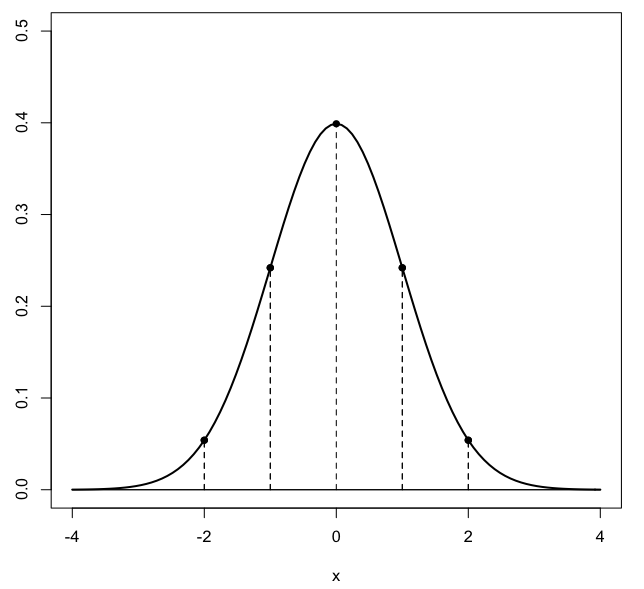
\includegraphics [scale=0.4] {gauss3.png} \end{center}
\begin{document}
\maketitle
\Large
This short write-up has notes on the various "laws" in electromagnetism, and basic derivations on the components used in circuits (resistor, capacitor, inductor).
\subsection*{Gauss's Law}
There are two different laws from Gauss.  The first one is for electric charge, and relates the distribution of charge to the flux of the electric field.  It can be written in a differential form using the divergence, and in a surface integral form.
\[ \nabla \cdot \mathbf{E} = \frac{Q}{\epsilon_0}  \]
\[ \iint \mathbf{E} \cdot dA = \frac{Q}{\epsilon_0}  = \nabla \cdot \mathbf{E} \] 
The way this is used in practice is to construct a surface where the electric field is the same everywhere and normal to the surface.  For example, with a sphere with charge $Q$, evaluate the field on the surface of a second sphere at radius $R$ from the first.  Then 
\[ E \ 4 \pi R^2 = \frac{Q}{\epsilon_0}  \]
\[ E = \frac{Q}{\epsilon_0 4 \pi R^2}  \]



\vspace{2cm}
Gauss's Law for Magnetism


Coulomb's Law
Ampere's Law
Faraday's Law
\subsection*{Capacitor}
A simple capacitor consists of two electrical conductors (plates) separated by a dielectric (insulator).  A capacitor stores energy in the form of the electric field between the plates.  The potential difference is dependent on how much charge is present, and physical characteristics like the size and geometry of the plates and the distance between them.

The capacitance is the ratio of the electric charge on each conductor to the potential difference
\[ C = \frac{Q}{V} \]
The unit is the farad, which is equal to one coulomb per volt.  Typical values might be microfarads $\mu F$.

Uses of capacitors include their property that they block direct current, yet allow alternating current to pass.  In appropriate combinations, they can be used to tune a circuit to a particular resonant frequency (e.g. in a radio).

The energy stored in a capacitor can be calculated as the work done in moving a charge
\[ W = \int_0^Q V \ dq = \int_0^Q  \frac{q}{C} \ dq = \frac{1}{2} \frac{Q^2}{C}  \]
The integral here takes account of the fact that the voltage depends on how much charge is currently on the plates.

Since current does not actually flow across the capacitor, for each electron that leaves the positive plate, one must join the negative plate.  Charge is the integral of current with time
\[ i = \frac{dq}{dt} \]
\[ \int i \ dt = \int \frac{dq}{dt} \ dt = \int dq = Q = VC \]
In a DC circuit with a voltage and a resistor
\[ V_0 = i(t)R + \frac{1}{C} \int_{t_0}^t i(t) dt \]
\[ \frac{d}{dt} \ V_0 = 0 = R \frac{di}{dt} +  i(t) \]
\[ RC \ \dot{i} + i = 0 \]
The rate of change of $i$ is proportional to $i$.  This is just an exponential with


\subsection*{Inductor}
Inductor

\end{document}  